%\documentclass[journal,12pt,draftclsnofoot,onecolumn]{IEEEtran} %draftclsnofoot
%\documentclass[confl, draftclsnofoot]{IEEEtran}
%\documentclass[conference,onecolumn,draft]{IEEEtran}
\documentclass[conference, 12pt]{IEEEtran}
\usepackage{fancyhdr}
\usepackage{grffile}
\usepackage{color}
\usepackage{graphicx}
\usepackage{cite}
\usepackage{multicol}
\usepackage{subcaption}
\usepackage{algorithm}
\usepackage{algpseudocode}
\usepackage{pifont}
\usepackage{subcaption}
\usepackage{siunitx}
\usepackage{flushend}

%\usepackage{setspace}
%\doublespacing
%\onecolumn
\begin{document}
%
% paper title
% can use linebreaks \\ within to get better formatting as desired
    \title{
        Minimal Viable Waterworld Agents:\\
        Experimenting with MultiAgent Reinforcement Learning
    }
%
%
% author names and IEEE memberships
% note positions of commas and nonbreaking spaces ( ~ ) LaTeX will not break
% a structure at a ~ so this keeps an author's name from being broken across
% two lines.
% use \thanks{} to gain access to the first footnote area
% a separate \thanks must be used for each paragraph as LaTeX2e's \thanks
% was not built to handle multiple paragraphs
%

    \author{Michael Hegerhorst}

% note the % following the last \IEEEmembership and also \thanks -
% these prevent an unwanted space from occurring between the last author name
% and the end of the author line. i.e., if you had this:
%
% \author{....lastname \thanks{...} \thanks{...} }
%                     ^------------^------------^----Do not want these spaces!
%
% a space would be appended to the last name and could cause every name on that
% line to be shifted left slightly. This is one of those "LaTeX things". For
% instance, "\textbf{A} \textbf{B}" will typeset as "A B" not "AB". To get
% "AB" then you have to do: "\textbf{A}\textbf{B}"
% \thanks is no different in this regard, so shield the last } of each \thanks
% that ends a line with a % and do not let a space in before the next \thanks.
% Spaces after \IEEEmembership other than the last one are OK (and needed) as
% you are supposed to have spaces between the names. For what it is worth,
% this is a minor point as most people would not even notice if the said evil
% space somehow managed to creep in.


% The paper headers
%\markboth{Journal of \LaTeX\ Class Files,~Vol.~6, No.~1, January~2007}%
%{Shell \MakeLowercase{\textit{et al.}}: Bare Demo of IEEEtran.cls for Journals}
% The only time the second header will appear is for the odd numbered pages
% after the title page when using the twoside option.
%
% *** Note that you probably will NOT want to include the author's ***
% *** name in the headers of peer review papers.                   ***
% You can use \ifCLASSOPTIONpeerreview for conditional compilation here if
% you desire.


% If you want to put a publisher's ID mark on the page you can do it like
% this:
%\IEEEpubid{0000--0000/00\$00.00~\copyright~2007 IEEE}
% Remember, if you use this you must call \IEEEpubidadjcol in the second
% column for its text to clear the IEEEpubid mark.


% use for special paper notices
%\IEEEspecialpapernotice{(Invited Paper)}


% make the title area
    \maketitle
%copyright notice
% TODO
% \thispagestyle{plain}
% \fancypagestyle{plain}{
%   \fancyhf{} % clear all header and footer fields
%   \fancyfoot[L]{978-1-4673-8988-4/17/\$31.00~\copyright2017~IEEE} % change
%       copyright notice here if required
%   \renewcommand{\headrulewidth}{0pt}
%   \renewcommand{\footrulewidth}{0pt}
% }

    \begin{abstract}
        Efficient metabolism in bioengineered tissues requires a robust vascular system to provide healthy microenvironments to the cells and stroma. Such networks form spontaneously during embryogenesis from randomly distributed endothelial cells. There is a need to bioengineer endothelial cells so that network formation and operation is optimal for synthetic tissues. This work introduces a computational model that simulates \textit{de novo} vascular development and assesses the effectiveness of the network in delivering nutrients and extracting waste from tissue. A genetic algorithm was employed to identify parameter values of the vaculogenesis model that lead to the most efficient and robust vascular structures. These parameter values control the behavior of cell-level mechanisms such as chemotaxis and adhesion. These studies demonstrate that genetic algorithms are effective at identifying model parameters that lead to near-optimal networks. This work suggests that computational modeling and optimization approaches may improve the effectiveness of engineered tissues by suggesting target cellular mechanisms for modification. 

    \end{abstract}


% IEEEtran.cls defaults to using nonbold math in the Abstract.
% This preserves the distinction between vectors and scalars. However,
% if the journal you are submitting to favors bold math in the abstract,
% then you can use LaTeX's standard command \boldmath at the very start
% of the abstract to achieve this. Many IEEE journals frown on math
% in the abstract anyway.

% Note that keywords are not normally used for peerreview papers.
    \renewcommand\IEEEkeywordsname{Key Words}
    \begin{IEEEkeywords}
% TODO
% Synthetic biology, self organization, vascular development, tissue engineering,
%         genetic algorithms, optimization, bioengineering.
    \end{IEEEkeywords}

% For peer review papers, you can put extra information on the cover
% page as needed:
% \ifCLASSOPTIONpeerreview
% \begin{center} \bfseries EDICS Category: 3-BBND \end{center}
% \fi
%
% For peerreview papers, this IEEEtran command inserts a page break and
% creates the second title. It will be ignored for other modes.
%\IEEEpeerreviewmaketitle

% TODO
% \section{Introduction}
%
% Multicellular organisms depend on vascular systems for nutrient delivery and waste removal\cite{delindavis:bloodevolution}. These vascular networks are formed either through vasculogenesis, a biological process in which scattered vessel precursor cells self-organize to create new networks or through angiogenesis, in which new vessels sprout from the existing vessels.

Both vasculogenesis and angiogenesis are driven primarily by chemotaxis, a mechanism in which cells move in response to a chemical gradient, along with cell-cell adhesion \cite{delindavis:Merks2008ContactInhibited}. While many questions remain, progress in understanding and exploiting both vasculogenesis and angiogenesis is being made from a bioengineering perspective  \cite{Kaully2009VascularizationThe} \cite{Lovett2009Vascularization}. Dahl et al. \cite{delindavis:vascularnetworksinorgandevelopment} successfully implanted tissue-engineered vascular grafts in baboons and dogs. Melero-Martin et al. \cite{delindavis:bioengineeredvascularnetworks} showed that robust development of functional vascular networks is possible \textit{in vivo}.

With additional research in this area, bioengineered cells could be used to form functional vascular networks to create a useful delivery mechanism in synthetic tissues. However, to apply bioengineering approaches to vascular cells, genetic targets need to be identified that when modified, improve the effectiveness of the vascular systems that emerge. Given the vast number of possible targets, a method is required that could assist engineers in identifying those genetic targets.

This paper presents a proof-of-concept genetic algorithm approach to solving this problem. The genetic algorithm acts to modify a computational model of vascular network development embedded within a cell cultivation environment. The search space of the optimization are the values of model parameters which control the mechanisms of the vascular cells such as chemotaxis. Changing these parameters modifies the behavior of individual cells which ultimately influence the spatial organization of the emergent vascular network. To evaluate the quality of this network, the model simulates its operation by determining fluid flow through each vessel, and subsequent nutrient delivery to the cultured cells. The returned fitness value quantifies the total metabolic activity of culture by using bioengineered microbial cells and measuring the total product produced.

The paper is organized as follows. First, the computational model of de novo vascularization is described followed by a description of the genetic algorithm. Next, we present the results which show that genetic algorithms can identify parameter values that improve network quality. There follow details of how the network operation is simulated and the fitness function values calculated. The paper concludes with a discussion of the potential impact of this work and the remaining challenges which need to be solved to operationalize the technique.




%
% \section{Self Organizing Vascularization Model}
%
% \label{vascularModel}

\begin{figure*}[t]
    \begin{center}
        \begin{tabular}{m{6cm}m{6cm}}
            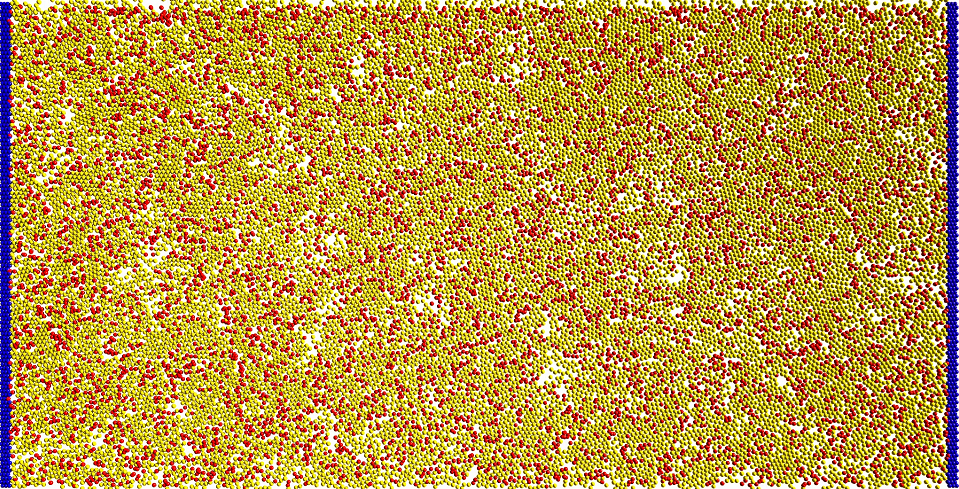
\includegraphics[width=5.9cm]{./figures/init_state.png} &
            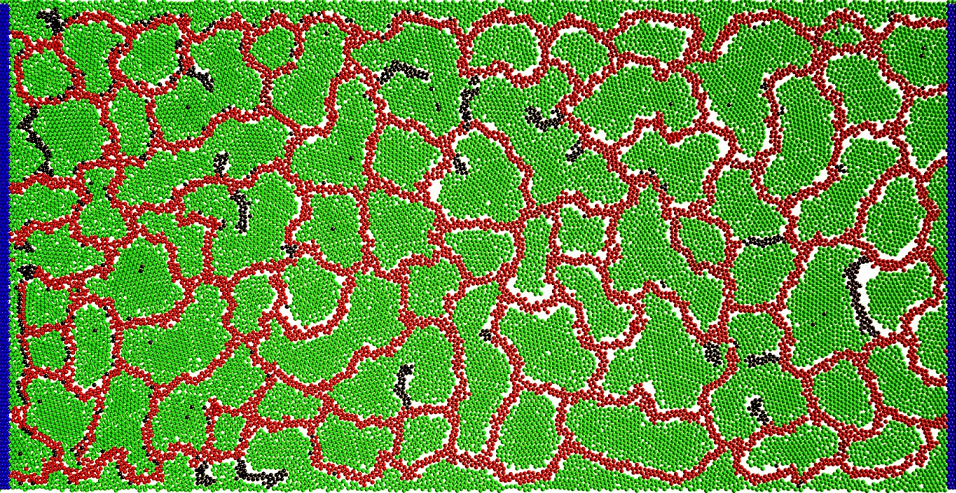
\includegraphics[width=5.9cm]{./figures/vessel30.png}\\
            (a) Initial random distribution      & (b) Stable vascular network
            \\
            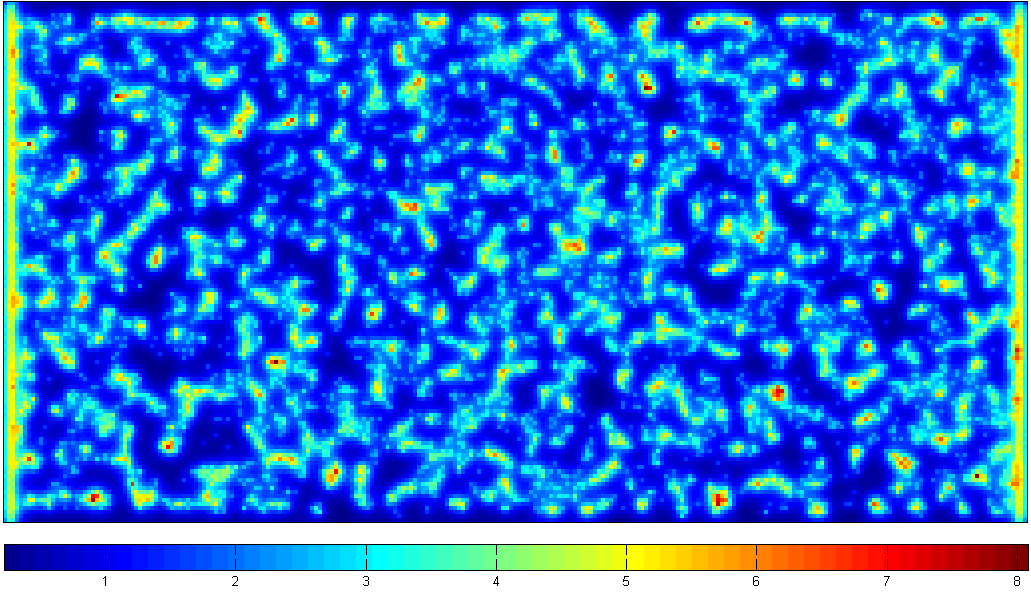
\includegraphics[width=5.9cm]{./figures/Chemo_init_state.png}
            \hspace{50mm} &
            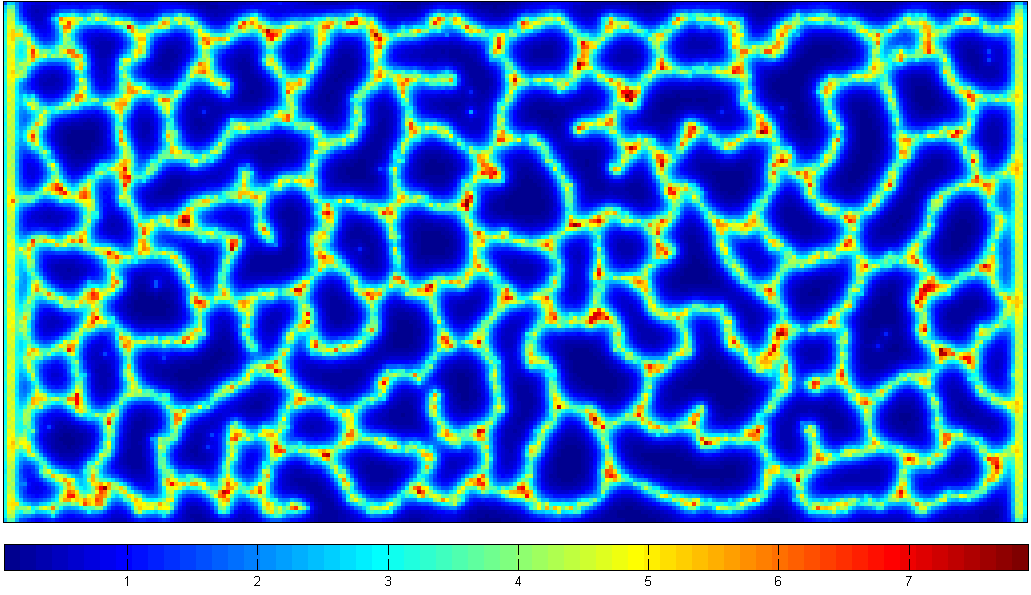
\includegraphics[width=5.9cm]{./figures/Chemo_steady_state.png}
            \hspace{50mm}\\
            (c) Chemoattractant during formation & (d) Chemoattractant state
            distribution \\
        \end{tabular}
    \end{center}
    \caption{\textbf{Self-organizing Network}: (a) is the initial conditions with
    fixed circulatory cells (blue) on each side and vascular (red) and supported
    cells (yellow) randomly mixed; (b) is the steady state network following self
    organization; (c) is the distribution of chemoattractant during vessel formation
    and (d) is at a steady state. In all images of biochemical distribution, blue
    signifies a low concentration, while red signifies a high concentration.}
    \vspace{+1mm}
    \label{phaseOne}
\end{figure*} 

At this proof-of-concept stage, a two-dimensional model was constructed and evaluated. Figure~\ref{phaseOne}(a) illustrates the initial state of the simulated cell culture. Vessel cells (blue) that simulate the external circulatory system are arranged in two columns on both sides of the cell culture area. The left column represents the source, and the right column represents the sink, in parallel to the arterial-venous network architecture in vertebrates \cite{delindavis:arterialvenoussystems}.

The tissue to be supported by the vascular network is simplified to be a field of identical cells, referred to as supported cells (yellow), randomly distributed across the area in between the two circulatory cell columns. Mixed within this field of supported cells are vascular cells (red), similar  to the endothelial cells in vertebrates \cite{delindavis:Merks2008ContactInhibited}. It is the mechanisms of the vascular cells that are to be optimized by the genetic algorithm.

During simulation, the randomly distributed vascular cells self-organize and can form a vascular network connected to both columns of circulatory cells. If this process succeeds, the supported cells will form clusters contained within each network lacuna. An example of a self-organized network is illustrated in Figure~\ref{phaseOne}(b). This developmental process is described in more detail in Section~\ref{vesselDevelopment}.

To evaluate the performance of the network, first an estimate of the flow through the vascular system is calculated and then the vascular network operation is simulated. As the network provides nutrients, the supported cells become active (turn green in the figures) and consume nutrients and secrete wastes. Note that in this case the network fitness would be high because almost all of the supported cells are active and close to a vessel. This network operational process is described in more detail in Section~\ref{fitnessFunction}.

\subsection{De Novo Vascularization Model}
\label{vesselDevelopment}

The two key cellular mechanisms in vascularization are chemotaxis, where cells move in respond to chemical gradients, and tight junctions, where adjacent cells form strong bonds.  Cells are modeled as particles that can secrete and respond to chemicals and move in response to forces. The modeling framework is based on iDynamics \cite{Lardon2011IDynoMiCS} originally created for biofilm models.

Initially, the particles representing epithelial cells are placed randomly in the simulation domain mixed with the support cells.  A chemotactic nutrient is initially supplied at concentration $N_{c}$, set at $8.9 \times 10^{-8} m^{-2}$.  The fixed cells on the sides of the cell culture secrete $C_{long}$, a chemoattractant with small decay rate, and $C_{short}$, a chemoattractant with a large decay rate. The moving cells within the culture only secrete $C_{short}$. The decay rates affect the shape of the chemoattractant gradient. $C_{short}$ is a localized concentration with a sharp gradient, and $C_{long}$ has a long-distance shallow gradient.  The concentrations of each are described by the Monod-kinetic reaction in Equation \ref{chemoattractantsecretion}.  $D_{c}$ of both chemoattractants are set to $1 \times 10^{-13} m^{2} s^{-1}$ as given in the \text{in-vitro} angiogenesis study of Merks et al \cite{delindavis:Merks2008ContactInhibited}; $\beta$ is the decay rate; $M$ is the mass of the secreting cell; $k$ is the Monod-kinetic coefficient; $\mu$ is the maximum secretion rate.

\begin{equation}
\frac{\partial C}{\partial t}=D_{c}\bigtriangledown^{2} C + \mu \frac{N_c}{(N_c +k)} M - \beta C
\label{chemoattractantsecretion}
\end{equation}

The moving cells respond to the gradient of the chemoattractants by tending to towards higher concentrations in a process described in Equation 2 and by Adler \cite{delindavis:chemotaxisbasepaper}. Let $p$ be a particle that responds to chemoattractant $C$. A random unit vector $\vec{c}$ is generated and considered as a potential chemotactic force on $p$. The local gradient of chemoattractant across $p$ in direction $\vec{c}$ is determined by sampling $C$ ahead of $p$, referred to as $C^{+}$, and behind $p$, referred to as $C^{-}$. The magnitude of force $F$ in direction $\vec{c}$ is given by the equation \ref{chemotaxis} \cite{delindavis:Merks2008ContactInhibited}, where $\lambda$ is the parameter that controls the magnitude of the response to the gradient and $\alpha$ controls saturation of the chemotactic force. The force $F$ is only applied to the particle if greater than zero.

\begin{equation}
F = \lambda \Big(\frac{C^{+}}{1 + \alpha C^{+}} - \frac{C^{-}}{1 + \alpha C^{-}}\Big)
\label{chemotaxis}
\end{equation}



Adhesive forces act among the particles and are attractive at close distances and neutral otherwise. In this work, endothelial cell-cell adhesion is strong and endothelial-supported cell is weak. When endothelial cells become close, tight junctions begin to form, binding the cells together as a precursor to vessel construction. In the model, if two adjacent cells form a tight junction, then a stiff spring connects the corresponding particles.

In addition to chemotactic force $F \cdot \vec{c}$, each particle experiences forces due to non-overlapping constraints caused by competition for space. Once the net forces have been assigned to each particle, the system is relaxed by a shoving algorithm which moves the particles along their force vectors to minimize stress. In this way, the vessel particles push through the supported particles, form clumps due to attractive chemotactic forces, and then buckle and extend immature vessels. The system can eventually reach the morphology illustrated in Figure~\ref{phaseOne}(b), in which all biomechanical forces are relaxed, and concentrations of molecules are stable, see Figure~\ref{phaseOne}(d).

\begin{table}[ht]
\caption{Known parameter descriptions} % title of Table
\centering
\begin{footnotesize}
\begin{tabular}{l l l}
\hline
Parameter   &  Value & Description\\ \hline \hline
%\\ [1ex]      % [1ex] adds vertical space
$D_{c}$     & $1 \times 10^{-13} m^{2} s^{-1}$ & Chemoattractant Diffusion coefficient \\%% value verified - cgl
$N_{c}$     & $3 \times 10 g L^{-1}$ & Chemoattractant nutrient concentration \\%% value verified - cgl
$M_{fixed}$  & $1 \times 10^{-11} g$ & Mass of fixed epithelial cells \\%% value verified - cgl
$M_{moving}$  & $1 \times 10^{-11} g$ & Mass of moving epithelial cells \\%% value verified - cgl
$\alpha $     &  $0.1$           & Saturation of chemotactic force\\
[1ex]      % [1ex] adds vertical space

\hline
\end{tabular}
\end{footnotesize}
\label{parameters}
\end{table}

%
% \section{The Genetic Algorithm}
%
% The self organizing vascular model has seven parameters with unknown values
(Table~\ref{unknownparameters}). The best fit for these parameters was found using a
genetic algorithm from the Java Genetic Algorithms Package
\cite{cgl:meffert2011genetic}. The seven parameters are used as genes in individual
chromosomes. The initial population had a size of three and was constructed by random
selection of parameter values from the ranges shown in Table~\ref{unknownparameters}.
As the population evolves during runs of the genetic algorithm, each individual is
evaluated using the parameter values encoded in the genes used to run the vascular
model (see Section~\ref{vascularModel} for more details). The resulting vascular
network is then evaluated as described in Section~\ref{fitnessFunction}, and the
fitness is assigned based on the metabolic production. Next, genetic operators were
run on the population followed by a re-evaluation of the population that now
contained new individuals. Finally, selection was applied to obtain the new
population for the next round of evolution.
Crossover and mutation operators were included in the genetic algorithm, with the
crossover operator applied to 35\% of the population per generation and the mutation
operator was applied to each gene with a probability of 1/12. An elitist ranking
selector cloned the top \%90 of the population, with the remaining 10\% of the
population filled with the same individuals in the order of fitness. The results
presented in this paper were obtained using 1000 steps of evolution.


\begin{table}[ht]
    \caption{Parameters searched by the GA} % title of Table
    \centering
    \begin{footnotesize}
        \begin{tabular}{l l l l}
            \hline
            Parameter         & Low        & High      & Description
            \\ \hline \hline
            $k$               & $10^{-10}$ & $10^{-2}$ & Monod-kinetic coefficient
            \\
            $\mu_{short}$     & $1$        & $7$       & Secretion rate of
            $C_{short}$           \\
            $\mu_{long}$      & $1$        & $7$       & Secretion rate of $C_{long}$
            \\
            $\beta_{short}$   & $10^{-5}$  & $10^{-1}$ & Decay rate of $C_{short}$
            \\
            $\beta_{long}$    & $10^{-10}$ & $10^{-3}$ & Decay rate of $C_{long}$
            \\
            $\lambda_{short}$ & $1$        & $6$       & Chemoattractant response to
            $C_{short}$ \\
            $\lambda_{long}$  & $1$        & $6$       & Chemoattractant response to
            $C_{long}$  \\
            \hline
        \end{tabular}
    \end{footnotesize}
    \label{unknownparameters}
\end{table}
%% Range Values from VNoptimization.java, VNFitnessFunction.java
%%
%% gene[0] = new DoubleGene(gaConf, 1, 6);                  lambda_short
%% gene[1] = new DoubleGene(gaConf, 1, 6);                  lambda_long
%% gene[2] = new DoubleGene(gaConf, 1, 7 );                 mu_short
%% gene[3] = new DoubleGene(gaConf, 1, 7 );                 mu_long
%% gene[4] = new DoubleGene(gaConf, 0.00001, 0.1 );         beta_short
%% gene[5] = new DoubleGene(gaConf, 0.0000000001, 0.001 );  beta_long
%% gene[6] = new DoubleGene(gaConf, 0.0000000001, 0.01);    k
%%


%
% \section{Results}
%
% Initial runs of the algorithm were performed on a two dimensional cellular culture.
Its height was set to 0.768 mm while the width was fixed at 1.536 mm. The total
number of supported and vascular cells were 4200 and 1800, respectively where
vascular cells contributed to 30 per cent of total number of cells. A total of 384
circulatory cells simulating the external delivery and metabolic product extraction
system is implemented as two identical columns on two sides of the cellular culture.
The number of all mentioned cells were kept constant through the experiment. The
simulations started with a random distribution of supported and vascular cells inside
the culture. Sixteen simulated hours are allocated for network development, after
which the network's quality is evaluated. If no path of vessels is found that
connects the source to the sink, then the fitness score is set at zero. Otherwise,
the fitness score of the network is estimated by measuring the metabolic productivity
of the supported cells while simulating the operation of the vascular network for two
simulated hours. This process is described in detail in Section~\ref{fitnessFunction}.


Figure~\ref{evolutions} shows the best case fitness of the networks produced during
the running of the genetic algorithm. The algorithm starts with random values for the
chosen parameter within the given ranges. As shown in the graph, the GA is
unsuccessful in creating a productive cell culture for the first several evolutions.
However, once it finds a parameter set leading to a functioning network, it
continually improves the quality of solutions. After 1,000 iterations, the highest
fitness level was 537.66 $\mu g$ of product production. The parameter values
contributing to the best case are shown in Table~\ref{results}.

\begin{figure}[!t]
    \centering
    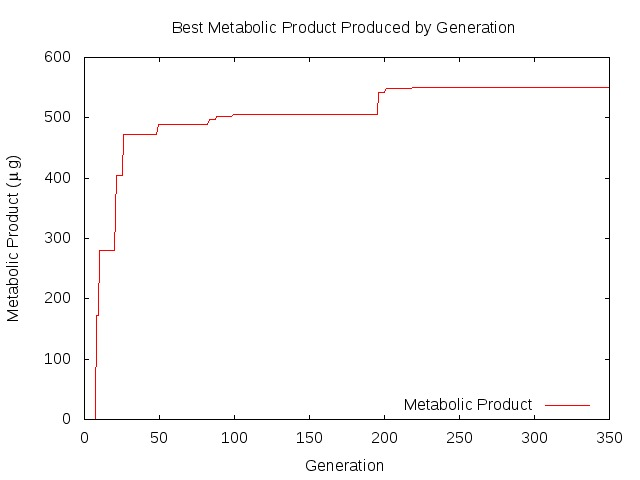
\includegraphics[width=3in]{./results/evolution products.jpg}

    \caption{The metabolic production of the best-so-far individual identified as a
    function of generation. Only a single run is provided due to the four hours
    needed for each fitness evaluation.}
    \label{evolutions}
\end{figure}



\begin{table}[ht]
    \caption{The best parameter values found by the GA} % title of Table
    \centering
    \begin{footnotesize}
        \begin{tabular}{l l l}
            \hline

%\\ [1ex]      % [1ex] adds vertical space
            $k$                & $6.78 \times 10^{-3}$ & Monod-kinetic coefficient
            \\
            $\mu_{short}$      & $5.12$                & Secretion rate of
            $C_{short}$           \\
            $\mu_{long}$       & $6.10$                & Secretion rate of $C_{long}$
            \\
            $\beta_{short} $   & $67.3 \times 10^{-3}$ & Decay rate of $C_{short}$
            \\
            $\beta_{long} $    & $7.41 \times 10^{-6}$ & Decay rate of $C_{short}$
            \\
            $\lambda_{short} $ & $2.69$                & Chemoattractant response to
            $C_{short}$ \\
            $\lambda_{long} $  & $1.99$                & Chemoattractant response to
            $C_{long}$\\
            [1ex]      % [1ex] adds vertical space

            \hline
        \end{tabular}
    \end{footnotesize}
    \label{results}
\end{table}

\begin{figure*}[ht]
    \begin{center}
        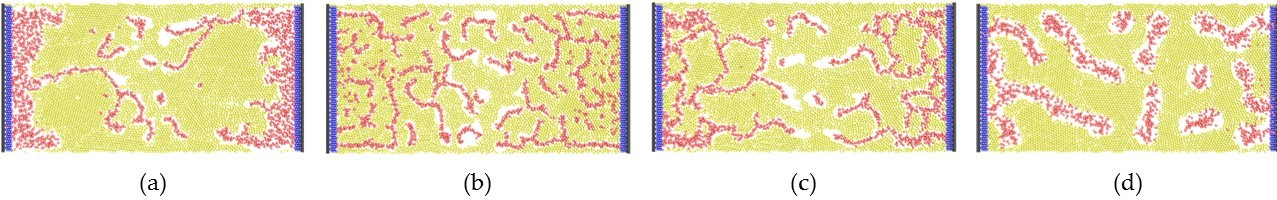
\includegraphics[width=\textwidth]{./results/bad factories.jpg}
    \end{center}
    \caption{Sample results of the GA during its evolution. These results show
    unsuccessful attempts of the GA at creating a consistent vascular network for the
    flow of nutrients and products}
    \label{badFactories}
\end{figure*}

\begin{figure*}[ht]
    \begin{center}
        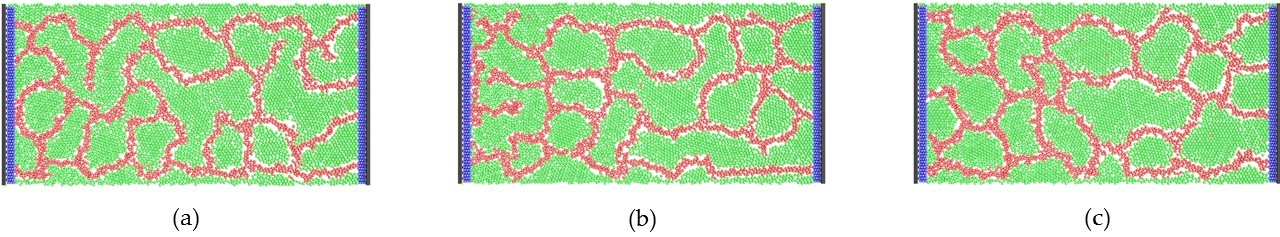
\includegraphics[width=\textwidth]{./results/good factories.jpg}
    \end{center}
    \caption{A sample of best solutions identified by the genetic algorithm during
    evolution. These results depict vascular networks that have successfully
    nourished the supported cells along with removing their products and waste}
    \label{goodFactories}
\end{figure*}

Figure~\ref{badFactories} shows some sample cell cultures produced by the genetic
algorithm during its evolution. As it is seen in the figure, some arrangements of the
vascular cells do not form a network for the flow of material and thus no production
is obtained in the system. Figure~\ref{badFactories}~(a) depicts a cell culture with
most of the vascular cells accumulated beside the circulatory cells on the sides and
occasional formations in the middle. This can be a result of high chemotactic
response to $C_{long}$ and $\alpha$.

Figures~\ref{badFactories}~(b) and (d) both demonstrate scattered and disconnected
lines of vascular cells floating among supported cells. Such arrangements result from
a low amount of $C_{long}$ but a high amount of $\beta_{short}$. It should be
mentioned that the cell culture in Figure~\ref{badFactories}~(d) has a higher
$\beta_{short}$ than the one in ~\ref{badFactories}~(b) which accounts for the
thicker lines of vascular cells. On the other hand, Figure~\ref{badFactories}~(c)
shows another unsupported cell culture with several cycles of vascular cells but no
path connecting the source to the sink. This result follows from low
$\lambda_{short}$ and high $\lambda_{long}$ and $\mu_{long}$.

Figure~\ref{goodFactories} depicts cellular cultures found by the GA that have
successfully formed networks of vascular cells and reached the highest amount of
production. No patches of yellow non-producing cells are present in these cell
cultures. As depicted, vascular cells have successfully formed a number of lacunae
that feed all supported cells available in the culture and move waste and products
away. More lacunae of vascular cells means availability of nutrients to more
supported cells and therefore, higher production. Investigating the parameters
leading to these solutions reveal an average amount of $\lambda_{short}$ and
$\lambda_{long}$ and low amounts of $\mu_{short}$, $\mu_{long}$, $\beta_{short}$,
$\beta_{long}$ and $k$. There are few unconnected branches stretching from a few
points which given a larger time frame could lead to more lacunae and even a higher
production. The exact amount of each parameter for cultures depicted in
Figures~\ref{badFactories} is given in Table~\ref{figure-param-table}. For comparison
purposes, the parameter values for Figure~\ref{goodFactories}(a) is also given in the
same table.

\begin{table*}[t]
    \renewcommand{\arraystretch}{1.3}
    \caption{Parameter Table Corresponding to cellular cultures depicted in
    Figures~\ref{badFactories} and ~\ref{goodFactories}}
    \label{figure-param-table}
    \centering
    \begin{tabular}{c||c||c||c||c||c||c||c}
        \hline
        \bfseries Culture             & \bfseries $\lambda_{short}$ & \bfseries
        $\lambda_{long}$ & \bfseries $\mu_{short}$
        & \bfseries $\mu_{long}$
        & \bfseries $\beta_{short} $
        & \bfseries $\beta_{long}$
        & \bfseries $k$
        \\
        \hline\hline
        Figure~\ref{badFactories}-(a) & 1.28                       & 4.09
        & 5.90                   & 6.58                  & $6.79 \times 10^{-2}$
        & $5.96 \times 10^{-4}$
        & $2.64 \times 10^{-3}$
        \\
        Figure~\ref{badFactories}-(b) & 1.28                       & 5.92
        & 5.90                  & 5.21                  & $6.79 \times 10^{-2}$      & $8.54 \times 10^{-4}$
        & $8.96 \times 10^{-3}$
        \\
        Figure~\ref{badFactories}-(c) & 1.11                       & 1.22                      & 6.69                   & 4.50                  & $9.90 \times 10^{-2}$     & $2.06 \times 10^{-4}$
        & $1.49 \times 10^{-3}$
        \\
        Figure~\ref{badFactories}-(d) & 5.73                       & 1.22                      & 6.69                   & 4.50                  & $8.14 \times 10^{-2}$     & $5.70 \times 10^{-4}$
        & $2.17 \times 10^{-3}$
        \\
        Figure~\ref{goodFactories}    & 2.69                       & 1.34                       & 3.85                  & 6.10                  & $3.23 \times 10^{-2}$   & $7.68 \times 10^{-5}$
        & $2.64 \times 10^{-4}$
        \\
        \hline
    \end{tabular}
\end{table*}


%
% \section{Fitness of a Vascular System}
% \label{fitnessFunction}
%
% \begin{figure*}[ht]
    \begin{center}
        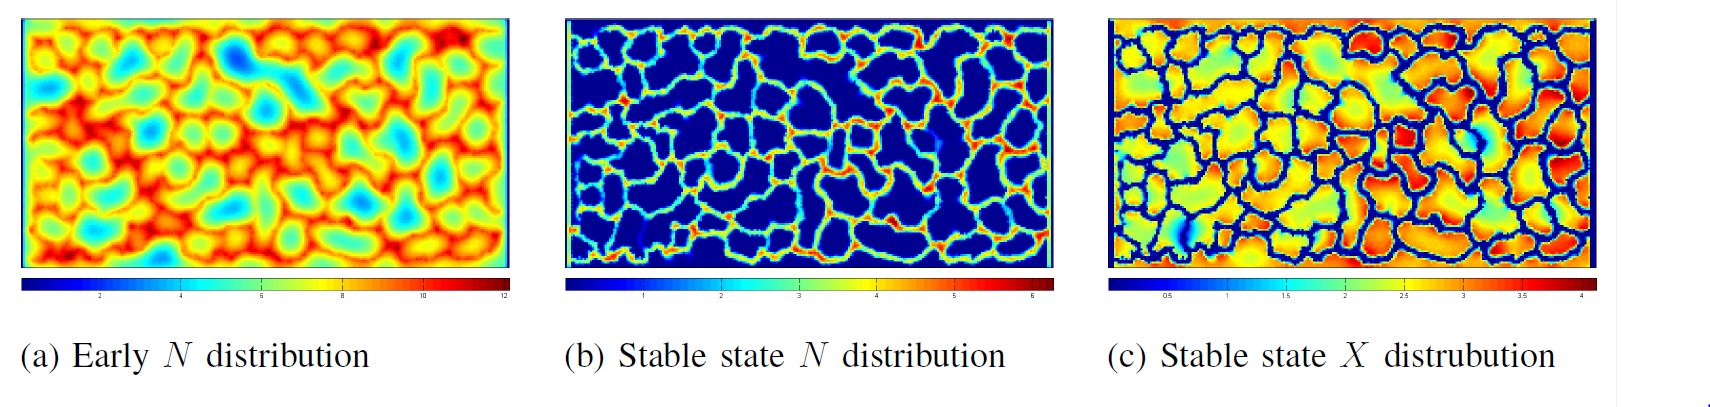
\includegraphics[width=\textwidth]{./figures/Figure7.JPG}
    \end{center}
    \caption{\textbf{Cell culture activation}: The distribution of nutrient (a) when
    the vessel flow begins, but the supported cells are not yet active, (b) at steady
    state nutrient distribution when the supported cells are active; note that all
    extra-vessel nutrient is consumed, (c) the product distribution when the
    supported cells are active.}
    \vspace{+1mm}
    \label{runningFactory}
\end{figure*}

The quality of the network is evaluated by determining the flow through each branch
and modeling the release of nutrients and the capture of secretions from the
supported cells. A full description of the functioning vascular model and its
derivation is given in \cite{Davis2017Exploiting}. To assess the health of the
supported cells given a running vascular network, the rate of metabolism of each
supported cell is estimated by measuring how efficiently the cells produce some
arbitrary product, $X$, described by Equation~\ref{productProduction}.

\begin{equation}
    \frac{\partial X}{\partial t}=+\mu _{p}  \frac{N}{(N+k_p)} \frac{k_i}{(X+k_i)}
    M_p + D_{p}\bigtriangledown^{2} X
    \label{productProduction}
\end{equation}

Where $M_p$ is supported cell biomass. To produce a realistic model of cellular
metabolism, the parameter values of the supported cells is replicated from
\cite{delindavis:Bernard1999Mass} and is based on vanillin production of Pycnoporus
cinnabarinus. The product $X$ is secreted by the supported cells consuming nutrient
$N$ following Michaelis-Menten kinetics with a reaction rate of $\mu _{p}$, where the
saturation of enzymes involved in the $X$ production is considered $k_p$. The
negative feedback due to product inhibition is also taken into account, with a
correspondent inhibitor constant $k_i$ \cite{Han1988Extended},
\cite{Levenspiel1980Monod} and \cite{Aiba1968Kinetics}.

%\input{modelTable}

Nutrient will be consumed by the supported cells in direct correspondence to the
production of $X$, but at a different reaction rate $\mu_n$:

\begin{equation}
    \frac{\partial N}{\partial t}=-\mu _{n}  \frac{N}{(N+k_p)} \frac{k_i}{(k_i+X)}
    M_p + D_{p}\bigtriangledown^{2} N
    \label{nutrientConsumption}
\end{equation}

Figure~\ref{runningFactory} illustrates the distribution of nutrient and product
during simulated network operation for the network illustrated in
Figure~\ref{phaseOne}(c).
Figure~\ref{runningFactory}(a) illustrates the nutrient distribution before the
supported cells have become active. In Figure~\ref{runningFactory}(b) gives the
nutrient distribution following supported cell activation. In
Figure~\ref{runningFactory}(c) the distribution of the product is illustrated. Note
the regions of low product (the blue areas) where the vascular flow is limited.

The final step is to integrate the amount of $X$ extracted from the cellular culture
by the vascular network over a fixed period, in this case two hours. This
accumulation of product will be a function of the aggregate metabolic rate of the
supported cells. It is this value the simulator returns as the fitness score of the vascular network architecture.





%
% \section{Discussion}
% This work explored a solution to the problem faced by bioengineers to determine those
cellular mechanisms to target for modification when improving vascularization for
synthetic tissue engineering. The method integrated a hybrid particle-based model of
vascularization as a fitness function with a genetic algorithm applied to optimize
the search space of model parameter values. The method is generic in that models of
different biological systems could be substituted for vascularization and the fitness
function likewise changed to reflect alternative objectives, such as minimizing
vascular function to combat tumor growth in cancer \cite{Mahoney2010MultiObjective}.

In this initial study, the search space was reduced to only consider parameters that
influence the chemotactic mechanism of the vascular cells. Previous work with the
model identified the importance of adhesion and tight junction formation in robust
network formation. However, increasing the number of parameters to include these
cellular mechanisms would significantly increase the search space, resulting in many
more fitness function calls. Given the modeling framework employed here
\cite{Lardon2011IDynoMiCS}, this is currently impractical because each fitness
evaluation takes at least four hours of CPU time running on a 3.6~GHz machine.
Recently two fast large-scale simulation systems have been developed by Ghaffarizadeh
et al. \cite{ghaffarizadeh2015agent} and \textsl{Biocellion}
\cite{delindavis:biocellion}. Both these systems implement an individual-based
approach similar to \textsl{cDynoMiCs} employed here. \textsl{Biocellion} is
implemented as a distributed architecture executable on the Cloud
\cite{Hashem2015Rise} and is capable of simulating complex 3D models of billions of
cells in a matter of a few hours. \textsl{Biocellion} has the potential to simulate
vascularization quickly enabling the optimization of more complex bioengineered
multicellular systems.

The principle challenge in bringing this work to practicality is to operationalize
the link between model parameters and actual genetic sequences. If this can be
achieved, then the output of the optimization process could be directly mapped to
engineering targets in the genome. In traditional bioengineering where products are
produced in biofactories \cite{delindavis:Sharma2001Production},
\cite{delindavis:vanDijl2013Bacillus}, targets are identified through analysis of
detailed metabolic models of microbial cells, such as \cite{Karp2015Pathway}. The
functioning of mammalian cells is less understood, particularly mechanisms such as
chemotaxis that are unrelated to metabolic processes, which can be modeled using flux
balance analysis.

The key to operationalizing bioengineering of multicellular systems is to utilize
multiscale models of the biological system under study. Multiscale models link the
mechanisms acting at different spatial and temporal scales together into an
integrated system where changes in expression and regulation of genes are manifested
in large-scale multicellular outcomes \cite{Martins2010Multiscale},
\cite{JosephWalpole2013Multiscale} \cite{Yu2016Multiclass}. If such detailed models
were employed, the high-level abstract parameters of this work would be replaced by
specific genetic mechanisms resulting in solutions being mapped directly to genetic
targets.



%
% \section{Conclusions}
% This work has shown that genetic algorithms are sufficiently powerful to optimize complex biological systems, even when there is a non-linear relationship between the parameters and the fitness function. This method can be applied to models of different biological systems that consider alternative objectives.

Many challenges exist before this optimization approach can be applied to actual bioengineered tissues. Two principle challenges are that (a) the speed of the simulations needs to be increased to allow expansion of the parameter space and to increase the fidelity of the model, and (b) methods to engineer the molecules that influence vascular tissue organization to meet the predicted optimal parameter values must be expanded and improved. However, although not all the molecules considered in this work can yet be easily tuned to meet optimal parameter values, existing real-world approaches are available for at least some of them. For example, the secretion rate of the chemoattractants can potentially be altered by changing the intracellular stability of genetically engineered chemoattractants guided by the N-end rule \cite{Varshavsky2011Nend}.  Similarly, there is the possibility of increasing the decay rate of both the short-range and long-range chemoattractants by adding selective targets of specific proteases that could be introduced into the culture system. Exploring these modifications may move this in silico system to an in vitro system with practical applications.




    \bibliographystyle{plain}

    \begin{small}

        \bibliography{references}

    \end{small}


\end{document}


